\documentclass[11pt]{article}
\usepackage[utf8]{inputenc}
\usepackage[spanish, es-tabla]{babel}
\usepackage{amssymb,amsmath,amsthm,amsfonts}
\usepackage{calc}
\usepackage{graphicx}
\usepackage{natbib}
\usepackage{url}
\usepackage[strings]{underscore}
\usepackage{parskip}
\usepackage{fancyhdr}
\usepackage{vmargin}
\usepackage{xcolor}
\usepackage{booktabs}
\usepackage{array}
\usepackage{float}
\usepackage{listings}
\usepackage{hyperref}
% Márgenes
\setmarginsrb{2 cm}{1.7 cm}{2 cm}{2.5 cm}{1 cm}{1 cm}{1 cm}{1 cm}
% Encabezados y pie de página
\pagestyle{fancy}
\fancyhf{}
\rhead{\IfFileExists{logo_di.png}{\includegraphics[scale=0.21]{logo_di.png}}{\textbf{UTFSM -- DII}}}
\lhead{\parbox[t]{0.72\textwidth}{\raggedright
\textbf{ICN292:} Sistemas de Información para la Gestión\\
\textbf{Profesores:} José Miguel González Paul / José Luis Sáez Tamayo\\
\textbf{Estudiante:} Sergio Cerecera}}
\cfoot{\thepage}
% Estilo para código SQL
\definecolor{codegreen}{rgb}{0,0.55,0.2}
\definecolor{codegray}{rgb}{0.45,0.45,0.45}
\definecolor{codepurple}{rgb}{0.5,0.1,0.7}
\definecolor{backcolour}{rgb}{0.97,0.97,0.98}
\definecolor{sqlblue}{rgb}{0.0,0.2,0.7}
\lstdefinestyle{sqlstyle}{
backgroundcolor=\color{backcolour},  
commentstyle=\color{codegreen}\itshape,
keywordstyle=\color{sqlblue}\bfseries,
numberstyle=\tiny\color{codegray},
stringstyle=\color{codepurple},
basicstyle=\ttfamily\footnotesize,
breakatwhitespace=false,  
breaklines=true,  
captionpos=b,  
keepspaces=true,  
numbers=left,  
numbersep=7pt,  
showspaces=false,  
showstringspaces=false,
showtabs=false,  
tabsize=2,
frame=single,
rulecolor=\color{black!15}
}
\lstset{style=sqlstyle}

% Formato de encabezados, manteniendo una jerarquía simple y uniforme
\setlength{\headheight}{42pt}
\setcounter{secnumdepth}{0}
\makeatletter
\renewcommand{\section}{\@startsection{section}{1}{0pt}
  {-1.2ex plus -.5ex minus -.2ex}
  {0.7ex plus .2ex}
  {\normalfont\large\bfseries}}
\renewcommand{\subsection}{\@startsection{subsection}{2}{0pt}
  {-0.9ex plus -.3ex minus -.2ex}
  {0.4ex plus .1ex}
  {\normalfont\normalsize\bfseries}}
\makeatother
\hypersetup{
colorlinks=true,
linkcolor=sqlblue,
urlcolor=sqlblue
}
\begin{document}
% ---------------------------------------------------------
% PORTADA Y ENCABEZADO
% ---------------------------------------------------------
\begin{center}
\vspace*{0.2cm}
{\Large \textbf{Laboratorio 4: Base de Datos Austral Editores}}\\[0.2cm]
{\large \textbf{Consultas SQL e Ingeniería Inversa Relacional}}\\
{\normalsize Segundo Semestre 2026}\\
\vspace{0.3cm}
\textbf{Repositorio Público GitHub:}\\
\url{https://github.com/tu-usuario/ICN292-Lab4-Cerecera-Sergio}
\end{center}
\vspace{0.25cm}
% ---------------------------------------------------------
% ENTREGABLE 1
% ---------------------------------------------------------
\section{Entregable 1: Modelo Entidad--Relación}
A partir de la ejecución del script DDL se procedió a la reconstrucción del esquema de base de datos relacional \texttt{austral} mediante la herramienta de ingeniería inversa (\textit{Reverse Engineer}) en MySQL Workbench.
El modelo implementado consta de cuatro entidades principales:
\begin{itemize}
\item \textbf{autores:} Entidad fuerte que almacena el identificador primario (\texttt{id_autor}), nombre, país de origen y género literario principal. Actúa como tabla padre para libros y pagos.
\item \textbf{colecciones:} Registra las líneas editoriales de publicación (\texttt{id_coleccion}), con su título y fecha oficial de lanzamiento.
\item \textbf{libros:} Entidad dependiente vinculada mediante claves foráneas hacia \texttt{autores} ($1:N$) y \texttt{colecciones} ($1:N$), registrando métricas de volumen, páginas y ejemplares comercializados.
\item \textbf{pagos:} Entidad transaccional vinculada a \texttt{autores} ($1:N$), que almacena los montos y fechas de liquidación financiera hacia los autores.
\end{itemize}
\begin{figure}[H]
\centering
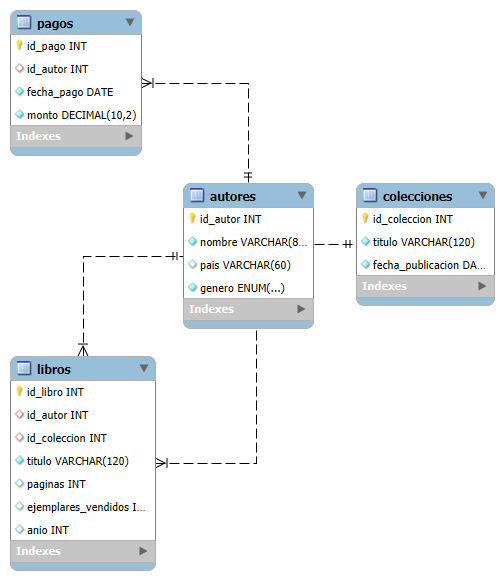
\includegraphics[width=0.88\textwidth]{ICN292-Lab4-Cerecera-Sergio.png}
\caption{Diagrama Entidad--Relación generado mediante ingeniería inversa en MySQL Workbench.}
\label{fig:eer_austral}
\end{figure}
\vspace{0.25cm}
% ---------------------------------------------------------
% ENTREGABLE 2
% ---------------------------------------------------------
\section{Entregable 2: Consultas SQL}
\subsection{Consulta 1: Filtrado de autores con lógica trivaluada}
\noindent\textbf{Justificación conceptual:} En SQL rige la lógica trivaluada (\textit{Three-Valued Logic - 3VL}), donde una evaluación puede resultar en \texttt{TRUE}, \texttt{FALSE} o \texttt{UNKNOWN}. Cuando un atributo contiene el valor nulo (\texttt{NULL}), cualquier comparación convencional como \texttt{pais <> 'Chile'} evalúa estrictamente a \texttt{UNKNOWN}. Dado que la cláusula \texttt{WHERE} únicamente conserva registros cuya condición evalúa a \texttt{TRUE}, los autores con país no definido son omitidos automáticamente a menos que se incorpore la condición explícita \texttt{OR pais IS NULL}.
\begin{lstlisting}[language=SQL]
SELECT nombre, genero
FROM autores
WHERE pais <> 'Chile' OR pais IS NULL
ORDER BY nombre ASC;
\end{lstlisting}
\begin{figure}[H]
\centering
\includegraphics[width=0.72\textwidth]{consulta-01.png}
\caption{Autores extranjeros o sin país registrado.}
\end{figure}
\subsection{Consulta 2: Rango cerrado de extensión de páginas}
Se seleccionan los títulos y número de páginas de aquellas obras cuya extensión se sitúa en el intervalo cerrado de 190 a 220 páginas mediante el operador \texttt{BETWEEN}, ordenadas ascendentemente.
\begin{lstlisting}[language=SQL]
SELECT titulo, paginas
FROM libros
WHERE paginas BETWEEN 190 AND 220
ORDER BY paginas ASC;
\end{lstlisting}
\begin{figure}[H]
\centering
\includegraphics[width=0.72\textwidth]{consulta-02.png}
\caption{Obras comprendidas entre 190 y 220 páginas.}
\end{figure}
\subsection{Consulta 3: Métricas agregadas del catálogo}
Se calculan las estadísticas globales del catálogo mediante las funciones de agregación \texttt{COUNT}, \texttt{SUM}, \texttt{AVG}, \texttt{MIN} y \texttt{MAX}, asignando alias legibles a cada columna.
\begin{lstlisting}[language=SQL]
SELECT
COUNT(*) AS total_libros,
SUM(ejemplares_vendidos) AS total_ejemplares_vendidos,
AVG(paginas) AS promedio_paginas,
MIN(anio) AS anio_mas_antiguo,
MAX(ejemplares_vendidos) AS max_ejemplares_vendidos
FROM libros;
\end{lstlisting}
\begin{figure}[H]
\centering
\includegraphics[width=0.88\textwidth]{consulta-03.png}
\caption{Resumen agregado del catálogo de libros.}
\end{figure}
\subsection{Consulta 4: Géneros literarios sin duplicados}
Consulta para listar los géneros literarios presentes en el registro de autores, suprimiendo repeticiones mediante la cláusula \texttt{DISTINCT} y ordenando en sentido alfabético.
\begin{lstlisting}[language=SQL]
SELECT DISTINCT genero
FROM autores
ORDER BY genero ASC;
\end{lstlisting}
\begin{figure}[H]
\centering
\includegraphics[width=0.55\textwidth]{consulta-04.png}
\caption{Géneros literarios únicos registrados.}
\end{figure}
\subsection{Consulta 5: Autores con múltiples publicaciones en 2024}
Se cruzan las tablas \texttt{autores} y \texttt{libros} para determinar aquellos escritores con más de una obra registrada durante el año 2024, agrupando por identificador de autor y filtrando los agregados con \texttt{HAVING}.
\begin{lstlisting}[language=SQL]
SELECT
a.nombre,
COUNT() AS libros_2024
FROM autores a
JOIN libros l ON a.id_autor = l.id_autor
WHERE l.anio = 2024
GROUP BY a.id_autor, a.nombre
HAVING COUNT() > 1
ORDER BY a.nombre ASC;
\end{lstlisting}
\begin{figure}[H]
\centering
\includegraphics[width=0.62\textwidth]{consulta-05.png}
\caption{Autores con más de un libro publicado en 2024.}
\end{figure}
\subsection{Consulta 6: Obras destacadas de 2024}
Extracción de los tres títulos con mayor volumen de ventas comercializados durante el año 2024 que superan el umbral de 2.000 unidades, utilizando ordenamiento descendente y \texttt{LIMIT 3}.
\begin{lstlisting}[language=SQL]
SELECT titulo, ejemplares_vendidos
FROM libros
WHERE anio = 2024 AND ejemplares_vendidos > 2000
ORDER BY ejemplares_vendidos DESC
LIMIT 3;
\end{lstlisting}
\begin{figure}[H]
\centering
\includegraphics[width=0.68\textwidth]{consulta-06.png}
\caption{Top 3 de ventas del año 2024.}
\end{figure}
\subsection{Consulta 7: Ciclo de inserción y eliminación controlada}
Se documenta la verificación previa a la remoción del registro \textit{Papel Mojado} y la posterior constatación del vaciado de la tupla tras invocar la sentencia \texttt{DELETE}.
\begin{lstlisting}[language=SQL]
-- 1. Insercion del libro
INSERT INTO libros (id_autor, id_coleccion, titulo, paginas, ejemplares_vendidos, anio)
VALUES (3, 2, 'Papel Mojado', 260, 50, 2024);
-- 2. Comprobacion previa
SELECT * FROM libros WHERE titulo = 'Papel Mojado';
-- 3. Eliminacion
DELETE FROM libros WHERE titulo = 'Papel Mojado';
-- 4. Comprobacion posterior
SELECT * FROM libros WHERE titulo = 'Papel Mojado';
\end{lstlisting}
\begin{figure}[H]
\centering
\includegraphics[width=0.7\textwidth]{consulta-07-previo.png}
\caption{Verificación previa de la tupla antes de la ejecución del DELETE.}
\end{figure}
\begin{figure}[H]
\centering
\includegraphics[width=0.7\textwidth]{consulta-07-posterior.png}
\caption{Comprobación posterior: la consulta retorna 0 filas confirmando el borrado.}
\end{figure}
\subsection{Consulta 8: Actualización calculada de ventas}
Se efectúa la modificación acumulativa sobre la obra \textit{Cielo de Enero}, incrementando 100 unidades sobre el stock reportado. Se aporta la evidencia en tres fases: lectura inicial (1.500), mensaje de confirmación del motor en la consola de salida y lectura final (1.600).
\begin{lstlisting}[language=SQL]
-- 1. Verificacion previa
SELECT titulo, ejemplares_vendidos
FROM libros
WHERE titulo = 'Cielo de Enero';
-- 2. Modificacion calculada
UPDATE libros
SET ejemplares_vendidos = ejemplares_vendidos + 100
WHERE titulo = 'Cielo de Enero';
-- 3. Verificacion posterior
SELECT titulo, ejemplares_vendidos
FROM libros
WHERE titulo = 'Cielo de Enero';
\end{lstlisting}
\begin{figure}[H]
\centering
\includegraphics[width=0.65\textwidth]{consulta-08-previo.png}
\caption{Comprobación previa con el valor base de 1.500 ejemplares.}
\end{figure}
\begin{figure}[H]
\centering
\includegraphics[width=0.7\textwidth]{consulta-08-update.png}
\caption{Consola Action Output informando 1 fila afectada tras el UPDATE.}
\end{figure}
\begin{figure}[H]
\centering
\includegraphics[width=0.65\textwidth]{consulta-08-posterior.png}
\caption{Comprobación posterior reflejando el incremento a 1.600 ejemplares.}
\end{figure}
\subsection{Consulta 9: Cruce relacional de libros y colecciones}
Mediante un \texttt{INNER JOIN} se asocian los libros con su respectiva colección, extrayendo el título de la obra, el nombre de la serie y la fecha formal de publicación.
\begin{lstlisting}[language=SQL]
SELECT
l.titulo AS titulo_libro,
c.titulo AS titulo_coleccion,
c.fecha_publicacion
FROM libros l
JOIN colecciones c ON l.id_coleccion = c.id_coleccion;
\end{lstlisting}
\begin{figure}[H]
\centering
\includegraphics[width=0.88\textwidth]{consulta-09.png}
\caption{Listado de obras vinculadas a su respectiva colección editorial.}
\end{figure}
\subsection{Consulta 10: Cruce relacional y consolidación de pagos}
Se divide en dos etapas: primero el detalle de cada desembolso emitido a los autores, y segundo la suma total percibida por autor agrupada mediante \texttt{GROUP BY} y ordenada de forma descendente.
\begin{lstlisting}[language=SQL]
-- 1. Detalle transaccional de pagos
SELECT
a.nombre,
p.fecha_pago,
p.monto
FROM autores a
JOIN pagos p ON a.id_autor = p.id_autor;
-- 2. Consolidado total por autor
SELECT
a.nombre,
SUM(p.monto) AS total_pagado
FROM autores a
JOIN pagos p ON a.id_autor = p.id_autor
GROUP BY a.id_autor, a.nombre
ORDER BY total_pagado DESC;
\end{lstlisting}
\begin{figure}[H]
\centering
\includegraphics[width=0.7\textwidth]{consulta-10-detalle.png}
\caption{Detalle transaccional individual de pagos por autor.}
\end{figure}
\begin{figure}[H]
\centering
\includegraphics[width=0.65\textwidth]{consulta-10-totales.png}
\caption{Totales consolidados y ordenados por monto acumulado descendente.}
\end{figure}
\end{document}
